A search for the decay \btodsphi was published in \Ref{LHCb-PAPER-2012-025}, where all mentions of
the \phii meson refers to the $\phi(1020)$.
The decay \btodsphi proceeds via the annihilation of the constituent quarks of a \Bp meson
forming a virtual \Wp boson, in the \sm.
To achieve the final state, the \Wp decays into a $\cquark\squarkbar$ pair and an additional
\ssbar pair must be created from the \QCD field.
This is the only diagram that can perpetuate such a decay at tree level, because the initial state
quarks are all different to those in the final state.
A Feynman diagram for such a decay in the \sm
is shown in \Fig{fig:dsphi:feyn}.
The final state mesons can be formed in the way indicated, or the \ssbar pair from the \QCD field
can form the \phii, although this is colour suppressed.
Also, the gluon that forms the \ssbar pair can originate from any of the initial or final state
quarks.

Annihilation decays of \Bp mesons are rare in the SM due to the magnitude of
$|\V{ub}|\sim4\e{-3}$ (see \Eq{eq:th:vub}).
In fact, no fully hadronic decays proceeding via annihilation-type diagrams have yet been
observed.


\begin{figure}
  \begin{center}
    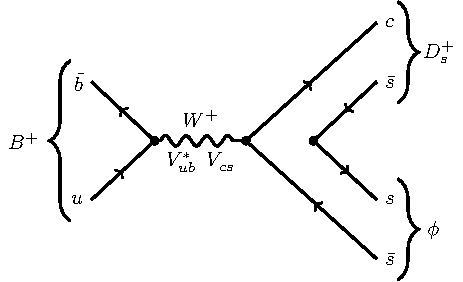
\includegraphics[scale=1]{feynman_dsphi_sm}
    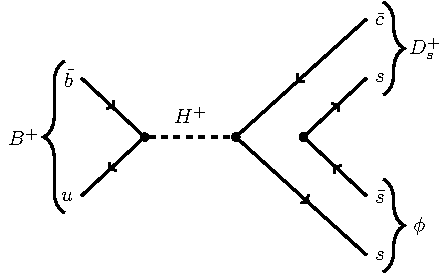
\includegraphics[scale=1]{feynman_dsphi_susy}
    \caption[Feynman diagram for the decay \btodsphi]
    {
      A Feynman diagram for the decay \btodsphi being mediated by a
      (left) \Wp in the SM, and
      (right) $H^+$ in SUSY.
      The \ssbar pairs shown here are formed from a gluon that can come from any quark.
      The arrangement of quarks forming the final state mesons shown is the colour favoured decay
    }
    \label{fig:dsphi:feyn}
  \end{center}
\end{figure}


%and SUSY, where the \ssbar pair are produced by a decaying gluon which could have
%originated from any of the four quarks.
%If the gluon were to be from one of the initial state quarks then the assumption of factorization
%does not hold.

Predictions for the branching fraction $\BF\big(\btodsphi\big)$ are calculated using the OPE defined
by the effective Hamiltonian~\cite{Zou:2009zza,Mohanta:2002wf,PhysRevD.76.057701,Lu:2001yz}:
\begin{equation}
  \Ham{eff}=
  -4\frac{G_F}{\sqrt{2}} \V{ub}\Vconj{cs}
  \big[
    C_1(\Lambda)\Op{1}+C_2(\Lambda)\Op{2}
    \big]
\end{equation}
where
\begin{align}
  \Op{1} &= \big(\bquarkbar\gamma_\mu P_Lu\big) \big(\cquarkbar\gamma_\mu P_Ls\big) \nonumber\\
  \Op{2} &= \big(\bquarkbar\gamma_\mu P_Ls\big) \big(\cquarkbar\gamma_\mu P_Lu\big).
\end{align}
The Wilson coefficients $C_1$ and $C_2$ are defined at the scale $\Lambda=m_b$,
and the projection operators are defined as $P_L=\tfrac12(1-\gamma_5)$ and
$P_R=\tfrac12(1+\gamma_5)$.
The short distance operators \Op{1} and \Op{2} both describe the transition $b\!\to scu$.
Despite the relatively simple effective Hamiltonian, \QCD effects limit the accuracy of calculating
the relative branching fraction $\BF\big(\btodsphi\big)$.

Beyond uncertainties in \V{ub}, predictions for the branching fraction $\BF(\btodsphi)$ in the \sm
range from
\approx$1\e{-7}$ to
\approx$7\e{-7}$~\cite{Zou:2009zza,Mohanta:2002wf,PhysRevD.76.057701,Lu:2001yz}.
The large range in branching fraction predictions is testament to the difficulties in the
theoretical calculation.
Calculating the decay dynamics is further complicated because the decay \btodsphi is not fully
factorizable, since the \ssbar pair can come from the final state quarks (the factorizable part) or
the initial quarks.
In the case that the gluon is emitted from an initial state quark the final state is
non-factorizable, becuase the hadronization component is not separable from the the short-range,
iteration, process.
There are also inherent uncertainties in the hadronic form-factors that describe the hadronization
process of the final state quarks.

Significant enhancements, beyond the \sm uncertainty, in $\BF\big(\btodsphi\big)$
could be observed were the decay to be mediated by additional \bsm
particles, particularly other charged bosons.
For example, in a model with \twoHDM --- such as \SUSY --- the decay \btodsphi
would be mediated by a charged Higgs $H^+$, this is shown in \Fig{fig:dsphi:feyn}.
More particles mean more Feynman diagrams that could add to the total amplitude.
Reference~\cite{Mohanta:2002wf} makes predictions for the branching fraction of the decay
\btodsphi in the \sm, as well as in a model with \twoHDM and a model with
\rpv:
%\bam{Smaller number is improved factorization}
\begin{align}
  %\BF\big(\btodsphi\big)_\mathrm{SM}&=0.67\e{-6}, \nonumber\\
  %\BF\big(\btodsphi\big)_\mathrm{2HDM}&=\pz8.0\e{-6}, \nonumber\\
  %\BF\big(\btodsphi\big)_\mathrm{RPV}&=3.06\e{-4}.
  %\BF\big(\btodsphi\big)|{\makebox[\widthof{$_\mathrm{2HDM}$}][l]{$_\mathrm{SM}$}}
  %&=1.88\e{-6}, \nonumber\\
  \BF\big(\btodsphi\big)|{\makebox[\widthof{$_\mathrm{2HDM}$}][l]{$_\mathrm{SM}$}}
  &=0.67\e{-6}, \nonumber\\
  \BF\big(\btodsphi\big)|_\mathrm{2HDM}
  &=8.0\pz\e{-6}, \nonumber\\
  \BF\big(\btodsphi\big)|{\makebox[\widthof{$_\mathrm{2HDM}$}][l]{$_\mathrm{RPV}$}}
  &=3.06\e{-4}.
\end{align}
The above number for the \sm branching fraction was calculated using the \QCD improved
factorization method~\cite{Beneke:2000ry}, but to illustrate the difficulties in \QCD calculations,
the same paper quotes $1.88\e{-6}$ using the factorization approximation.
These numbers indicate that, while the exact \sm value of $\BF\big(\btodsphi\big)$ is not well
known, the value for models with additional mediating particles could be enhanced significantly.

The \CP asymmetry, \acp, of a process is defined in terms of decay rates of $B$ hadrons:
\begin{equation}
  \acp = \frac{\Gamma(\Bbar\!\to\xbar{f}) - \Gamma(B\!\to f)}
  {\Gamma(\Bbar\!\to\xbar{f}) + \Gamma(B\!\to f)}
\end{equation}
for some final state $f$.
A positive value of \acp would indicate a preference of the antimatter process, above the matter
process.
In the SM $\acp(\btodsphi)=0$, because the process only contains one phase, in \V{ub}, but
interference from \bsm physics diagrams could alter this significantly.
Predictions from \Ref{Mohanta:2002wf} are:
\begin{align}
  \acp\big(\btodsphi\big)|_\mathrm{2HDM}
  &\leq 59\,\%, \nonumber\\
  \acp\big(\btodsphi\big)|{\makebox[\widthof{$_\mathrm{2HDM}$}][l]{$_\mathrm{RPV}$}}
  &\leq 14\,\%.
  \label{eq:dsphi:acpdef}
\end{align}
So, both measurements of $\BF\big(\btodsphi\big)$ and $\acp\big(\btodsphi\big)$ could lead to
evidence of \np.

%Further motivation for studying the decay \btodsphi comes from the
%historical conflict between measurements of
%$|\V{ub}|_\mathrm{inc}$ and $|\V{ub}|_{\tau\nu}$, as described in \Sec{sec:bsm:faisec:bsm:fail}.
%Since the decay \decay{\Bp}{\taup\nu_\tau} is also an annihilation-type decay, it is possible that
%measurements of \btodsphi could shed light on the potential source of this discrepancy.
%However, the publication of this analysis, \Ref{Crivellin:2014zpa} asserts that the
%discrepancies cannot be explained by new physics, and is rather due to underestimated uncertainties
%in either theory or experiment.




\subsection{Other annihilation-type hadronic decays}
The annihilation of the \Bp meson can perpetuate numerous decays resulting in fully hadronic
states, including a charmed meson.
The decay \decay{\Bp}{\Dp\Kstarz} proceeds in the same way as
\btodsphi, but the former needs a \ddbar pair to be created from the \QCD vacuum, rather than an
\ssbar pair.
Similarly, the decay \decay{\Bp}{\Ds\Kstarzb} is identical to the \btodsphi excepting that instead
of \decay{\Wp}{\cquark\squarkbar} the \Wp decays into an $\cquark\dquarkbar$ pair.
The decays \decay{\Bp}{\Dp\Kstarzb} and \decay{\Bp}{\Ds\Kstarz} are non-trivial diagrams in the
\sm, and heavily suppressed, but have similar final states.
The same final states can also come from the annihilation of the constituent
quarks of the \Bc meson.

While the following chapter only discusses the search for the decay \btodsphi, these other
interesting decay modes are searched for in
\Ref{LHCb-PAPER-2012-025}.

































